\section{Аналитическая часть}

В данном разделе проведен анализ предметной области, формализированы данные,
а также проведен анализ существующих решений.

\subsection{Анализ предметной области}

Термин "база данных" не имеет точного определения, но стоит отметить несколько из них.


\textbf{База данных} \cite{bd-1} --- это совокупность данных, хранимых в упорядоченной форме, с целью
обеспечения доступа к этим данным и их использования каким-либо организационными
или прикладными процессам.

\textbf{База данных} --- это самодокументирования собрание интегрированных записей.

\begin{itemize}
    \item Запись --- это события, которые надо где-то хранить;
    \item интегрированных --- записи, которые имеют некоторую структуру.
\end{itemize}

Также необходимо определиться с типом базы данных. 
Всего существует два основных применения баз данных

\begin{enumerate}[label=\arabic*.]
    \item \textbf{OLAP} \cite{OLAP} --- это метод обработки данных, который используется для анализа
                    больших объемов данных.
    \item \textbf{OLTP} \cite{OLTP} --- это метод обработки транзакций, который используется для
                    выполнения операция в режиме реального времени.
\end{enumerate}

Из этих данных определений следует, что для поставленной задачи больше подойдет метод
OLTP, так как для обработки посетителей в магазине, требуется обработка в реальном времени.

Для выполнения курсовой работы, также необходимо выбрать систему управления базами данных.

\textbf{СУБД} --- это приложение обеспечивающее создание, хранение, обновление и поиск информации.

У систем управления базами данных существует классификация: 

\subsection{Классификация СУБД}

\subsubsection{По модели данных}

\subsubsubsection{Дореляционные}

\begin{enumerate}[label=\arabic*.]
	\item \textbf{Инвертированные списки} (файлы). БД на основе инвертированных списков представляет собой совокупность файлов, содержащих записи (таблиц). Для записей в файле определен некоторый порядок, диктуемый физической организацией данных. Для каждого файла может быть определено произвольное число других упорядочений на основании значений некоторых полей записей (инвертированных списков). Обычно для этого используются индексы. В такой модели данных отсутствуют ограничения целостности как таковые. Все ограничения на возможные экземпляры БД задаются теми программами, которые работают с БД. Одно из немногих ограничений, которое все-таки может присутствовать --- это ограничение, задаваемое уникальным индексом. 
	\item \textbf{Иерархическая модель} данных подразумевает что элементы, организованные в структуры, объединены иерархической или древовидной связью. В таком представлении родительский элемент может иметь несколько дочерних,
	а дочерний --- только один родительский.
	\item \textbf{Сетевые} --- могут быть представлены в виде графа; логика выборки зависит от физической организации данных.
\end{enumerate}

\subsubsubsection{Реляционные}

В отличие от вышеописанных, в данной модели не существует 
физических отношений между сущностями. 
Хранение информации осуществляется
в виде таблиц (отношений), состоящих из рядов и столбцов. 
Отношение имеет
имя, которое отличает его от имён всех других отношений.

Существует несколько типов реляционных моделей:

\begin{itemize}
	\item \textbf{Структурный} --- данные --- набор отношений.
	\item \textbf{Целостностный} --- отношения (таблицы) отвечают определенным условиям целостности.
	\item \textbf{Манипуляционный} --- манипулирования отношениями осуществляется средствами реляционной алгебры и/или реляционного исчисления.
\end{itemize}


\subsubsection{По архитектуре организации хранения данных}

\begin{enumerate}[label=\arabic*.]
	\item \textbf{Локальные} --- все части локальной СУБД размещаются на одном компьютере.
	\item \textbf{Распределенные} --- части СУБД могут размещаться на 2-х и более компьютерах. 
\end{enumerate}

\subsubsection{По способу доступа к БД}

\begin{enumerate}[label=\arabic*.]
	\item \textbf{Файл-серверные} --- при работе с базой, данные отправляются приложению, которое с ней работает, вне зависимости от того, сколько их нужно. Все операции --- на стороне клиента. Файловый сервер периодически обновляется тем же клиентом.
	\item \textbf{Клиент-серверные} --- вся работа на сервере, по сети передаются результаты запросов, гораздо меньше информации. Обеспечивается безопасность данных, потому что все происходит на стороне сервера.
	\item \textbf{Встраиваемые} --- библиотека, которая позволяет унифицированным образом хранить;
	большие объемы данных на локальной машине. Доступ к данным может происходить через SQL либо через 
	особые функции СУБД. Встраиваемые СУБД быстрее обычных клиент-серверных и не требуют установки
	сервера, поэтому востребованы в локальном ПО, которое имеет дело с большими объемами данных.
	\item \textbf{Сервисно-ориентированные} --- БД является хранилищем сообщений, промежуточных состояний, метаинформации об очередях сообщений и сервисах;
	\item Прочие --- пространственная, временная и пространственно-временная.
\end{enumerate}



\subsection{Пользователи системы}

В системе присуствуют три уровня пользователей.

\begin{enumerate}[label=\arabic*.]
    \item \textbf{Сотрудник магазина} --- пользователь, обладающим возможностями только просматривать
    сущность посетителей.
	\item \textbf{Охрана} --- пользователь, обладающий возможностями просматривать сущности: камер,
	украденных товаров, полок, посетителей.
	\item \textbf{Администратор} --- пользователь, обладающий возможностями изменения сущностей и полей
	базы данных, также есть доступен просмотр всех сущностей.
\end{enumerate}

На рисунке \ref{fig:anal:use-case} представлена диаграмма использования приложения.

\begin{figure}[ht!]
	\centering
	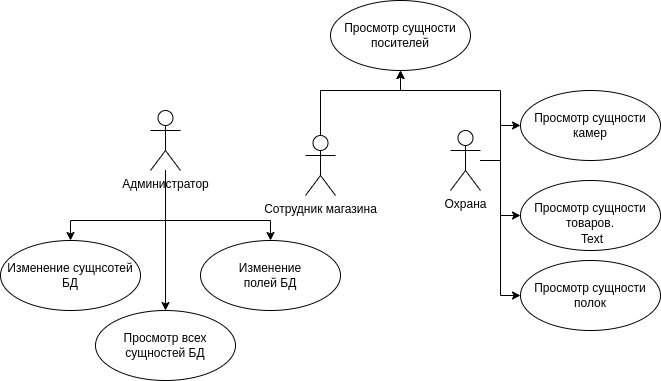
\includegraphics[width=0.7\linewidth]{assets/images/Use-case.drawio.png}
	\caption{Use-case диаграмма}
	\label{fig:anal:use-case}
\end{figure}
\FloatBarrier

\subsection{Формализация данных}

База данных состоит из нескольких таблиц:

\begin{enumerate}[label=\arabic*.]
	\item таблица посетителей Visitor;
	\item таблица камер Camera;
	\item таблица полок Shelf;
	\item талица товаров Product;
	\item таблица сетей магазинов Chain store;
\end{enumerate}

На рисунке представлена ER-диаграмма сущностей в нотации Чена.

\begin{figure}[ht!]
	\centering
	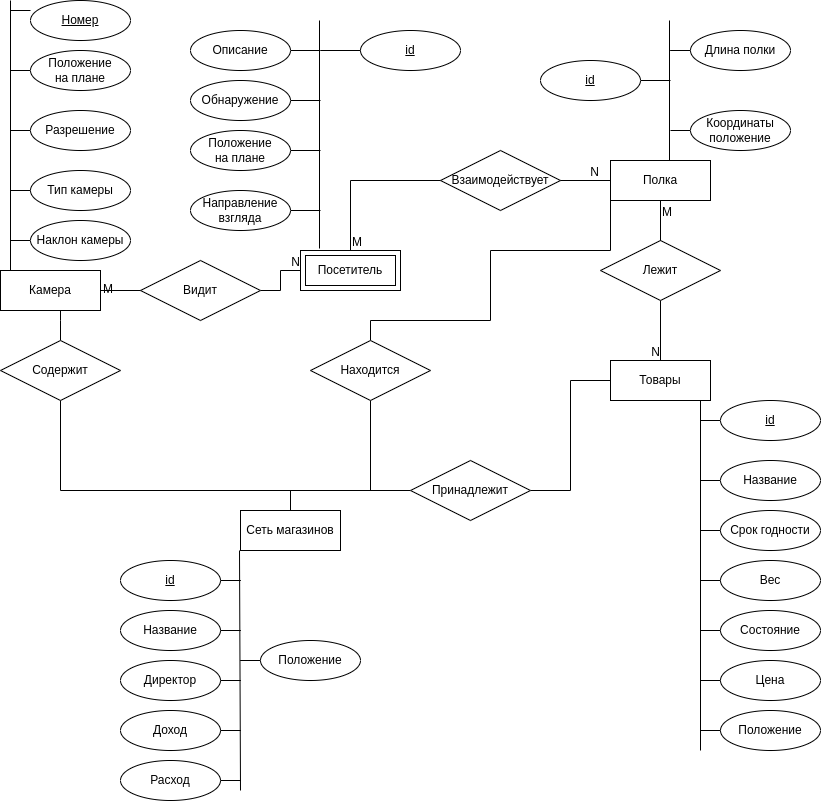
\includegraphics[width=0.9\linewidth]{assets/images/ER.drawio.png}
	\caption{ER-диаграмма в нотации Чена}
	\label{fig:anal:chen}
\end{figure}
\FloatBarrier

\subsection{Анализ существующих решений}

Среди уже имеющихся проектов, решающих поставленную задачу, были выделены 3 аналога.
Сравнение проводилось по ряду критериев, а именно наличие определения местоположения, 
не требующее дополнительного оборудования, определение характеристик посетителей.

В таблице \ref{decisions} представлено сравнение по вышеупомянутым критериям.

\begin{table}[ht!]
	\centering
	\caption{Существующие решения поставленной задачи}
	\label{decisions}
	\begin{tabular}{|p{2.6cm}|p{5cm}|p{4cm}|p{4cm}|}
			\hline
			\textbf{Название проекта} & \textbf{Местоположение} & \textbf{Доп. оборудование} & \textbf{Характеристики}\\
			\hline
			\textbf{Антивор \cite{Antivor}} & Определение местоположения может проводится при помощи дополнительного оборудования 
			& Требуется большое количество дополнительного оборудования для работы системы
			 & Не предусмотренно\\
			\hline

			\textbf{Воролов \cite{VOROLOV}} & Нет 
			& Оборудование не образует систему
			 & Не предусмотренно\\
			\hline

			\textbf{Navigine \cite{Navigine}} & Определение с помощью дополнительного оборудования 
			& Браслет и стационарный датчик
			 & С помощью браслета\\
			\hline
	\end{tabular}
\end{table}


Из таблицы можно сделать вывод, что каждая система требует большое количество дополнительного оборудования.
Также не во всех присутствует определение характеристик посетителей.

Создаваемое программное обеспечение предоставляет дополнительный функционал, без использования дополнительного оборудования.

Такими особенностями являются:

\begin{enumerate}[label=\arabic*.]
	\item определение местоположения на основе положения камер;
	\item задание характеристик посетителей;
	\item проверка взаимодействия посетителя и товара.
\end{enumerate}

\subsection{Выбор модели базы данных}

В данном проекте будет использоваться структурная реляционная модель данных, так как в рамках проектах
она обладает следующими преимуществами:


\begin{enumerate}[label=\arabic*.]
	\item изложение информации осуществляется с помощью таблиц;
	\item позволяет работать со структурированными данными;
	\item имеет возможность произвольного доступа к записям сущностей;
	\item исключает дублирование, при помощи реализации связи между отношениями посредством внешнего ключа.
\end{enumerate}

\subsection*{Вывод}

В данном разделе рассмотрены ролевые модели системы, конкретизированны хранимые данные и их
связь между собой, построенны соответствующие диграммы. Также представлено анализ существующих решений.
Был осуществлен выбор модели данных.